% --------------------------------------------------------------------------
% Template for WASPAA-2019 paper; to be used with:
%          waspaa17.sty  - WASPAA 2019 LaTeX style file, and
%          IEEEbib.bst - IEEE bibliography style file.
%
% --------------------------------------------------------------------------

\documentclass{article}
\usepackage{waspaa17,amsmath,amssymb,graphicx,url,times}
%\usepackage{waspaa17,amssymb,amsmath,graphicx,times,url}
\usepackage{color}
\usepackage{tabularx,booktabs,colortbl}
\usepackage{hyperref,subfig}
% Example definitions.
% --------------------
\def\defeqn{\stackrel{\triangle}{=}}
\newcommand{\symvec}[1]{{\mbox{\boldmath $#1$}}}
\newcommand{\symmat}[1]{{\mbox{\boldmath $#1$}}}

% Title.
% --------------------
\title{Estimation of Guitar String, fret and plucking position using a physical model and no training data}

%% Single addresses (uncomment and modify for single-address case).
%% --------------------
%\name{Author(s) Name(s)\thanks{Thanks to XYZ agency for funding.}}
%\address{Author Affiliation(s)}
%%
%% For example:
%% ------------
%%\address{School\\
%%       Department\\
%%       Address}
% ---------------
\name{Jacob~M\o ller Hjerrild, Silvin Willemsen and~Mads~Gr\ae sb\o ll~Christensen}%\thanks{Thanks to XYZ agency for funding.}}
\address{Audio Analysis Lab, CREATE, Aalborg University, Denmark\\
   \texttt{\{jmhh, sil, mgc\}@create.aau.dk}}
%


\begin{document}

\ninept
\maketitle

\begin{sloppy}

\begin{abstract}
  In this paper a method for analyzing guitar performances is proposed. This method extracts the activated string and fret as well as the plucking position, and it is purely based on a physical model of string excitation and vibration, hence it does not require any training data which makes it fast and effective. Since it operates on a 40 ms segment-by-segment basis it is suitable for real-time estimation...
\end{abstract}
%
\begin{keywords}
 Physical Modeling, Statistical Signal Processing, Parametric Pitch Estimation, Music Information Retrieval\vspace{-.8mm}
 \end{keywords}
%
\section{Introduction}
\label{sec:intro}
%
Recordings of music performances can be analyzed for various reasons, such as extracting stylistic details, artist recognition or detailed transcription of individual instruments, which can provide means for increasing usability of music learning technologies... 
% Specifically, the activated string and fret as
% well as the location of the plucking event along the guitar string are
% extracted from guitar signal recordings
\section{Problem Formulation}
The overall problem in this paper is the estimation of the guitar string, fret and plucking position without requiring any audio for training a model. The feature set is based on~\cite{hjerrild::icassp19} where pitch $\omega_0$ and inharmonicity $B$ is extracted with a parametric pitch estimator.  Instead of training a model from audio recordings, we propose a simulated model of guitar string vibrations based on physical properties such as dimensions and materials. Figure~\ref{fig:guitar_overview} gives an overview of the guitar, where 
\begin{figure}[h!]\
  \centering
  \centerline{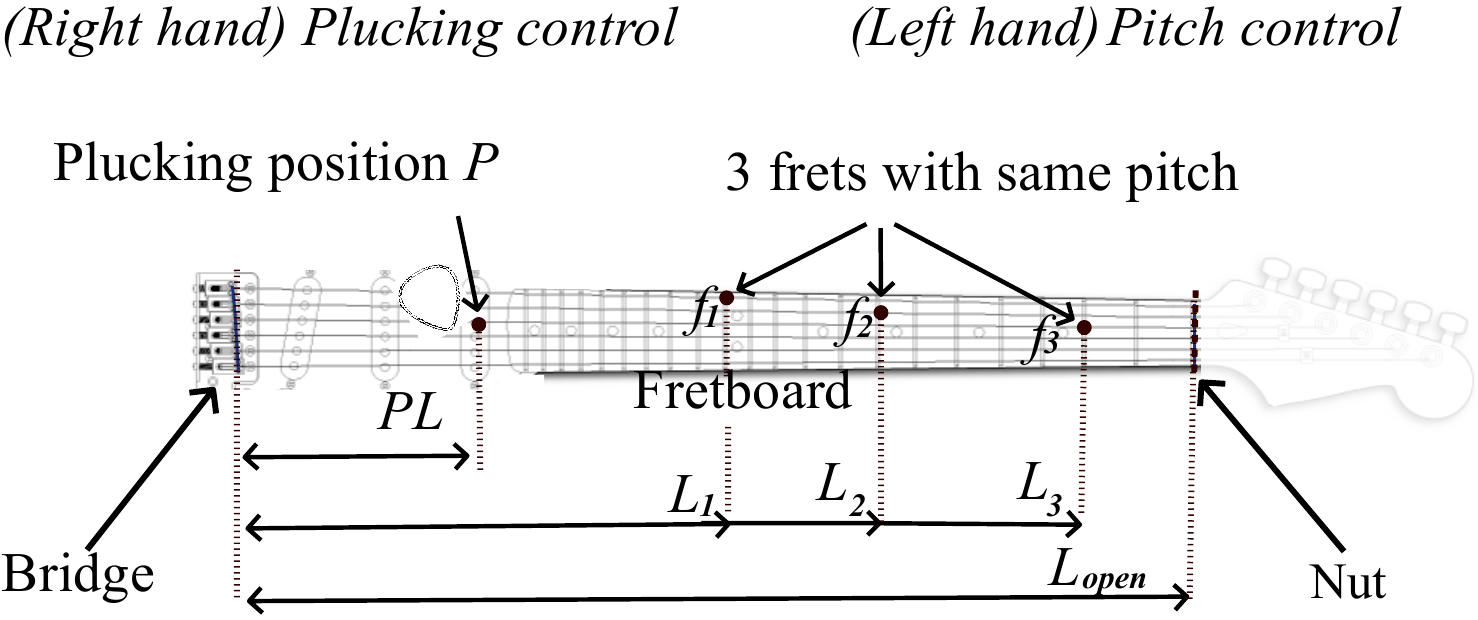
\includegraphics[width=1\columnwidth]{img/fender_drawing4.png}}
  \caption{The plucking position is controlled by the right hand while the left hand controls pitch using the fretboard. Similar pitch is produced in various positions. Source: Adapted from~\cite{phillips}.
  }\label{fig:guitar_overview}\vspace{-2mm}
\end{figure}
%
the right hand controls plucking position and the left hand controls pitch by using the fretboard. One pitch is produced in various positions and each string and fret combination is defined as one class, such that we have a set of $K$ mutually exclusive classes. 
%
%
%
% 
As demonstrated in~\cite{hjerrild::icassp19} a maximum likelihood classifier with a physically meaningful feature set consisting of pitch $\omega_0$ and inharmonicity $B$ can be utilized for distinguishing between string and fret combinations. 
Since the string is inharmonic the $m$th instantaneous frequency $\psi(\omega_0,B)$ is defined by the piano string model derived in~\cite{fletcher:piano_model} as 
%
\begin{equation}
  \psi_m(\omega_0,B) = m \omega_0 \sqrt{1+B m^2} \quad [s^{-1}], 
\end{equation}
where $\omega_0$ and $B$ can be estimated without detailed knowledge of the physics that defines the inharmonicity~\cite{ hjerrild::icassp19,abesser:automatic_string_detection_ml, barbancho:inharmonicity_tablature,michelson2018_aes}. 
However, modelling all classes on the guitar requires training data captured from each class. For 6 strings and 12 frets that is $K=72$  classes. Although~\cite{hjerrild::icassp19,barbancho:inharmonicity_tablature} shows that a fast training procedure requires only training data captured from one fret per string. There are three main challenges associated with such a a fast training procedure,%, which requires some work from the user. 
\begin{itemize}
    \item There is no information of class dependent distributions in the observed feature space, i.e. covariance structures. Except from the 6 classes represented in the training set.
    \item With only a few observations (i.e. 10 per string~\cite{hjerrild::icassp19}), it is impossible to conclude anything significant on the covariance structure of each class.
    \item Although training is relatively fast, it is required for every time for every different set of guitar strings.
%    \item  Can we eliminate the training procedure that requires recordings ?
%    \item  Can we extract the inharmonicity with higher precision based on the physical model of plucking ?
\end{itemize}
Can we eliminate the training procedure that requires the user to provide recordings and at the same time obtain a detailed and class dependent distributions in the feature space ? To overcome these problems, we will build a model from string material properties and dimensions. Detailed information of such properties are generally available on string packets.

%
%
%
%
%
%With detailed knowledge of the inharmonicity it is in fact possible to obtain a model for all frets on a string from one such model. In example, given the parameters $B_s( f_1 )$ and $\omega_{0,s}( f_1 )$ of the $s$th vibrating string for a given fret $f_1$, the corresponding parameter can be computed for any other fret $f_2$, using the inharmonicity model based on knowledge of the equal tempered scale as derived in~\cite{barbancho:inharmonicity_tablature}
%\begin{equation}
%    \widehat{B}_s( f_2 ) =  \widehat{B}_s( f_1 ) \: 2^{ \frac{  f_2 - f_1 }{ 6 }} = \frac{ \pi^3 E_s d_s^4 }{ 64 T_s L^2_{s}(f_2) } \quad [\cdot],
%\end{equation}
%where $E, d, T$ are the elastic Modulus, diameter and tension of the core which are considered constants and $L(f_2)$  is the length from the bridge to the given fret $f_2$.
%For the pitch estimates we have that the relation is
%\begin{equation}\label{eq:omega0_fast}
%  \widehat{\omega}_{0,s}( f_2 ) =  \widehat{\omega}_{0,s}( f_1 ) 2^{\frac{f_2-f_1}{12}} \quad [s^{-1}].
%\end{equation}
%
%
%
%
%
%
%
%
% 
\section{Inharmonic string model} \label{sec:string_model}
%
%\section{Proposed method}
%
In the following we discuss how to obtain such a model based only on physical string parameters, such we can exclude the requirement for training data, based on recordings.

\subsection{Inharmonic pitch definitions for the wrapped string}

In the following we derive the model of pitch and inharmonicity by assuming that we know the string length, diameter, material densities and tension.
The inharmonicity is highly correlated with the core diameter $d_c$ and string inharmonicity has been an area of research for more than a century see i.e.,~\cite{rayleigh:sound}. For string designers, it is in general desired to lower the inharmonicity. For low-pitched strings it is not desired to simply increase the core diameter in order to lower the fundamental frequency and therefore the strings are wrapped to add mass to the string and thus lower the inharmonicity along with the pitch. 

\noindent The mass per unit length $\mu$ of a string is defined by:

\begin{equation}
    \mu = \frac{\pi}{4}\Big(\rho_cd_c^2 + \rho_w\big[(2d_w+d_c)^2-d_c^2\big]\Big), \quad \bigg[\frac{kg}{m}\bigg],
\end{equation}
where $d_c$, $d_w$ are the diameters which relates to the diameter of the full string as $d_{\textup{full}}=2d_w+d_c$ and $\rho_c$, $\rho_w$ are the densities of the core and wrapping respectively. When the string is single-cored ($d_w = 0$), and thus not wrapped, the second term becomes zero. Since the tension mainly acts on the core, the string can be considered a single cored string having the same mass per unit length $\mu$, but with the diameter of the core $d_c$ only. The effective density of this theoretical material is defined as~\cite{firth:string_design} (with $\frac{\pi}{4}$ removed)
\begin{equation}
    \rho_{\textup{eff}} = \rho_c + \rho_w \big[(1+2\frac{d_w}{d_c})^2-1\big], \quad \bigg[\frac{kg}{m^3}\bigg].
\end{equation}

This effective density can be used to calculate the pitch for the string, from the tension and length. The relation between the string length $L_0$, the tension $T_0$ and the pitch $\omega_0$ is:

\begin{equation}
    T_0 = \pi (L_0\omega_0)^2d_c^2\rho_{\textup{eff}} = \mu(2L_0\omega_0)^2, \quad [N].
\end{equation}

It is clear that we can express the pitch with the well known equation:
\begin{equation}
    \omega_0 = \sqrt{\frac{T_0}{\mu}} \frac{1}{2L_0} \quad [s^{-1}],
\end{equation}
where the mass and length are being considered as constants. 
When the string is brought to pitch (tuned) it stretches according to its elastic modulus $E$ which is defined as
%
\begin{equation}\label{eq:tensile_stress}
    E = \frac{\text{Tensile stress}}{\text{Strain}}
   %= \frac{T_0/A_c}{\Delta L/(L_0 - \Delta L)} 
    = \frac{T_0 (L_0 - \Delta L)}{A_c \Delta L} \quad \bigg[\frac{N}{m^2}\bigg], 
\end{equation}
%
where $A_c = \frac{\pi d_c^2}{4}$ is the cross sectional area of the string-core, $E$, $A_c$ and $L_0$ are constants and $T_0$ and $\Delta L$ are proportional to each other. We use $L_0 - \Delta L$ in this formula to describe how much the string is stretched when brought to pitch and has the length from nut nut-to-bridge $L_0$.
%
%
%
%
\subsection{Calculating strain length $\Delta L$ from material properties}
%
It requires high precision to measure $\Delta L$ in a guitar string. It is, however, possible to calculate it from material constants. For the core of the string we can rewrite~\eqref{eq:tensile_stress}, i.e.,
%
\begin{equation}\label{eq:deltaL}
    \Delta L= \frac{L_0T_c}{A_cE + T_c}, \quad  [m], 
\end{equation}
%
where $T_c$ is the tension contributed by the core. For single-cored strings $T_c = T_0$.
%
The effect of wrapping on the tension is small, though not neglegible. We can assume the wrapping to be a spring with spring constant~\cite{childs:mechanical_engineering}
%
\begin{equation}\label{eq:k_wrapping}
    k = \frac{Gd_w^4}{8ND^3}, \quad \bigg[\frac{N}{m}\bigg]. 
\end{equation}
%
Here, $G$ is the shear modulus of the wrapping material, $N = \frac{L_0 - \Delta L}{d_w}$ is the number turns in the coil (assuming that for the untensioned string, every coil touches the previous and the next coil) and $D = d_c+d_w$ is the mean diameter of the spring~\cite{kemp:wound_and_unwound_strings}.
%
The length extension $\Delta L$ for a spring is
%
\begin{equation}\label{eq:deltaL_wrapping}
    \Delta L = \frac{T_w}{k}, \quad [m],
\end{equation}
%
where $T_w$ is the tension contributed by the wrapping. In~\eqref{eq:k_wrapping}, $k$ is (through variable $N$) dependent on $\Delta L$. Fortunately, we can rewrite the formula~\eqref{eq:deltaL_wrapping} to isolate $\Delta L$:
%
\begin{equation}
    \Delta L = T_w\frac{8(\frac{L_0 - \Delta L}{d_w})D^3}{Gd_w^4} = \frac{8T_wL_0D^3}{Gd_w^5 + 8T_wD^3} \quad [m].
\end{equation}
%
We know the desired tension $T_0$ for all strings. However, we can't fill this into the above formulas because the  the core and wrapping have a very different contribution on the total tension. We do know that $T_0 = T_c + T_w$, the total tension $T_0$ is the sum of the tension acting on the core $T_c$ and the tension acting on the wrapping $T_w$. Furthermore, we know that because the core and wrapping are part of the same string, they undergo the same length-extension $\Delta L$. We can thus set~\eqref{eq:deltaL} equal to~\eqref{eq:deltaL_wrapping}, i.e., 
%
\begin{equation}
    \Delta L = \frac{L_0T_c}{A_cE + T_c} = \frac{8D^3L_0T_w}{Gd_w^5 + 8D^3T_w} \quad [m].
\end{equation}
%
By inserting tension relations $T_c = T_0 - T_w$ and $T_w = T_0 - T_c$, the effect of the core and wrapping tensions are
%
\begin{equation}
    T_c = \frac{8A_cD^3ET_0}{Gd_w^5+8A_cD^3E}\text{ , } \newline
    T_w = \frac{GT_0d_w^5}{Gd_w^5 + 8A_cD^3E} \quad [N].
\end{equation}
%
An alternative way to calculate the contributions of $T_c$ and $T_w$ on the total tension is to compute their ratio $\tau_{c/w}$. This is defined as
%
\begin{equation}
    \tau_{c/w} = \frac{T_c}{T_w} = \frac{8A_cD^3E}{Gd_w^5}  \quad [\cdot] 
\end{equation}
%
and can be used to calculate by using $T_0 = T_c + T_w$ such that
%
\begin{equation}\label{eq:Tc_derived}
    %T_c (\frac{1}{\tau_{c/w}}+1) = T_0, \qquad T_w (\tau_{c/w} + 1) = T_0,  \\
    T_c = \frac{T_0}{\frac{1}{\tau_{c/w}}+1} \quad [N].
\end{equation}
%
Finally, inserting~\eqref{eq:Tc_derived} into~\eqref{eq:deltaL} (and/or filling in $T_w$ into~\eqref{eq:k_wrapping} for wrapped strings) gives the length extension based on the string-material properties of both core and wrapping. 
%
%
%
%
\subsection{Intrinsic and deflection caused inharmonicity}
Inharmonicity in instruments strings arises because of the presence of stiffness in the strings. Therefore, the partial amplitudes are not located as perfect multiples of the fundamental frequency.
The inharmonicity of each string arises from two sources, they are

1) Intrinsic inharmonicity due to the $\textbf{stiffness}$ of the string.

2) $\textbf{Stretching}$ of the string during plucking, which creates an initial pitch shift.

\noindent The intrinsic inharmonicity is~\cite{rossing:science_of_string_instruments}

\begin{align}
    B_i = \frac {\Delta f_i}{f} = \frac {K}{4} d_c^2  \quad [\cdot],
\end{align}

and the pitch shift for the maximum transverse displacement $\delta$ (pluck amplitude) is  

\begin{align}
    B_d = \frac {\Delta f_p}{f} = \frac {3K}{8} \delta^2 \quad [\cdot]. 
\end{align}

It is expected that $d<<\delta$; the pluck deflection is likely to be more than an order of magnitude greater than the string diameter. Hence, the pitch shift caused by plucking dominates the static string inharmonicity. This pitch shift is responsible for the initial twang of the string and dies down rapidly after the pluck. These two terms are related by $K$ which is

\begin{align}
    K = \frac {\pi^3 E d_c^2}{16 T L^2}, \quad [m^{-2}].
\end{align}

According to~\cite{fletcher:piano_model} the $\textit{intrinsic string inharmonicity}$ $B_i$ is

\begin{equation}
    B_i = \frac{\pi^2 E A R_g^2}{T L^2}, \quad [\cdot],
\end{equation}

where the radius of gyration $R_g^2 = \frac{I}{A} = \frac{\pi}{4}\big(\frac{d_c}{2}\big)^4 \frac{1}{A}$ assuming a one-dimensional - not planar - radius of gyration
%
\begin{equation}
    B_i =  \frac{\pi^3 E d_c^4}{64 T L^2} = \frac{\pi^2 E d_c^2}{64\rho_{\text{eff}} L^4 \omega_0^2}\quad [\cdot].
\end{equation}

The total inharmonicity is $B_i$ plus the inharmonicity caused by the transverse displacement

\begin{equation}
    B =  B_i + B_d =  \frac{\pi^3 E d_c^2(2d_c^2 + 3\delta^2)}{128 T L^2}\quad [\cdot] .
\end{equation}
%
\subsection{An MAP string and fret classifier}
Having found the pitch and the inharmonicity parameters $\boldsymbol{\phi} = [\widehat\omega_0, \widehat B ]^T$ from the observed signal snapshot $\mathbf{x} = [x(0), x(1), x(N-1)]^T$, the next problem is to classify the observed signal as being produced by a string and fret position. 
We have a set of $K$ mutually exclusive classes $\boldsymbol{\Gamma}=\{\gamma_1,\dots,\gamma_K\}$ representing all possible string and fret positions. The MAP-optimal classifier with decision function $\hat{\gamma}(\cdot): \mathbb{R}^I \rightarrow \boldsymbol{\Gamma}  $ is 
\begin{align}
    \hat\gamma_{{MAP}}(\boldsymbol{\phi}) &= \underset{\gamma\in\Gamma}{\operatorname{argmax}}\;{p(\gamma|\boldsymbol{\phi})} = \underset{\gamma\in\Gamma}{\operatorname{argmax}}\;{p(\boldsymbol{\phi}|\gamma)P(\gamma)}.
\end{align}
We model $\boldsymbol{\phi}$ as coming from a normal object with class $\gamma_k$, then the $k$th conditional probability density is   
\begin{equation}
    p(\gamma_k\lvert\boldsymbol{\phi}) =
    \mathcal{N}(\boldsymbol{\mu}_k,\,\boldsymbol{\Lambda}_k)\,
    %{{(2\pi)^{-1}\det{\boldsymbol{\Lambda}_k)^{\frac{-1}{2}}}}}\, \exp\bigg(\frac{-(\boldsymbol{\phi}-\boldsymbol{\mu}_k)^T\boldsymbol{\Lambda}_k^{-1} (\boldsymbol{\phi}-\boldsymbol{\mu}_k) }{2} \bigg),
\end{equation}
where the expectation vector $\boldsymbol{\mu}_k$ and covariance matrix $\boldsymbol{ \Lambda }_k$ is given from simulations, thus the covariance matrices are here modeled as being class dependent as compared to~\cite{hjerrild::icassp19}. 
%
There are several reasons for this. 
\begin{itemize}
    \item It is sufficient for accurate performance as shown in~\cite{hjerrild::icassp19} (i.e., electric gtr.: 97\%, acoustic gtr.: 100\%)
    \item It requires very little training data, something that is important due to the high number of classes formed by combinations of strings and frets. 
    \item Using a simple statistical model makes it possible to adapt the classifier to specific instruments using a simple training procedure.
\end{itemize}
%
Returning now to the classifier, neglecting terms that do not depend on the class index $k$ yields the following, classification scheme $\hat{\gamma}(\boldsymbol{\phi})={\gamma}_i$, with
%
\begin{equation}\label{eq:classifier}
%  \hat{\gamma}(\boldsymbol{\phi})={\gamma}_i \quad{\textup{with}}\quad 
  i=\underset{k=1,\dots,K}{\operatorname{argmax}}\;
\bigg\{ -\ln \lvert \boldsymbol{\Lambda}_k) \rvert + 2 \ln P(\gamma_k) - (\boldsymbol{\phi}-\boldsymbol{\mu}_k)^T \boldsymbol{\Lambda}_k (\boldsymbol{\phi}-\boldsymbol{\mu}_k)^T    %\frac{\left\lVert{\boldsymbol{\phi}-\boldsymbol{\mu}_k}\right\rVert^2}{\sigma^2} 
\bigg\}.
\end{equation}
%
%As can be seen, this classifier is the minimizer of the Euclidean distance between the observation and its expectation, with a correction factor of $2\sigma^2 P(\gamma_k)$. 
The prior $P(\gamma_k)$ can be specified from the number of training samples from class $\gamma_k$ or be assumed uniform, in which case it reduces to a maximum likelihood classifier, see i.e.,~\cite{mspr}.
%
\section{A Monte Carlo simulation based model}
In the following simulation, we model the feature space distributions based on physical parameters retaining to the string physics. Such parameters are given by string manufacturers and printed on the string package. In the following simulation the physical parameters of the strings are:
\begin{itemize}
    \item String length $\sim \mathcal{N}(L_0,\,\sigma_{L_0}^{2})$.
    \item String Tension $\sim \mathcal{N}(T_0,\,\sigma_{T_0}^{2})$.
    \item Plucking deflection $\sim \mathcal{N}(\delta,\,\sigma_{\delta}^{2})$.

    \item Core diameter $\sim \mathcal{N}(d_c,\,\sigma_{d_c}^{2})$.
    \item Core density $\sim \mathcal{N}(\rho_c,\,\sigma_{\rho_c}^{2})$.
    \item Wrapping diameter $\sim \mathcal{N}(d_w,\,\sigma_{d_w}^{2})$.
    \item Wrapping density $\sim \mathcal{N}(\rho_w,\,\sigma_{\rho_w}^{2})$.

\end{itemize}
%
%
%
%
\section{Evaluation} % (fold)
\label{sec:experiments}
%\vspace{-.6mm}
To evaluate the proposed plucking position estimator along with the string and fret classifier, some experiments have been conducted as described next. These experiments focus on segment-by-segment estimation and classification using short 40 ms segments, as this enables high-tempo and real-time applications of the proposed method. Hence, the experiments aim to demonstrate that this is possible.
%
%
%
% ---- EVALUATION 
%
%

\begin{table}\centering %\vspace{-1mm}
\caption{String and fret confusion matrix for the Martin  acoustic guitar. The classification errors are shown for each of the 6 strings.}
\label{tbl:string_confusion_martin}
\begin{tabularx}{0.46\textwidth}{@{}l*{7}{c}c@{}}
\toprule
Labels &Est. 6   &Est. 5 &Est. 4   &Est. 3   &Est. 2   &Est. 1   \\ 
\midrule
True 6   &130 \cellcolor[gray]{.8} &0  &0  &0  &0  &0  \\  
True 5   &0  & 130\cellcolor[gray]{.8} & 0   &0  &0  &0  \\
True 4   &0  &0  &130 \cellcolor[gray]{.8} &0  &0  &0  \\  
True 3   &0  &0  &0  &130 \cellcolor[gray]{.8} &0  &0  \\  
True 2   &0  &0  &0  &0  &130 \cellcolor[gray]{.8} &0  \\  
True 1   &0  &0  &0  &0  &0  &130 \cellcolor[gray]{.8} \\  
\bottomrule
\end{tabularx}
%\end{table}%\vspace{-.6mm}
%
%\begin{table}%\centering 
\vspace{6mm}
\caption{String and fret confusion matrix for the Firebrand electric guitar. The classification errors are shown for each of the 6 strings}
\label{tbl:str_confusion_firebrand}
\begin{tabularx}{0.46\textwidth}{@{}l*{7}{c}c@{}}
\toprule
Labels &Est. 6   &Est. 5 &Est. 4   &Est. 3   &Est. 2   &Est. 1   \\ 
\midrule
True 6   &130 \cellcolor[gray]{.8}       & 0                        &0      &0  &0  &0 \\
True 5   &5  & 125\cellcolor[gray]{.8}   & 0                        &0      &0  &0  \\
True 4   &0  &0  &122 \cellcolor[gray]{.8}                           & 8 &0  &0  \\
True 3   &0  &0  &3                     &127 \cellcolor[gray]{.8}   & 0   &0  \\
True 2   &0  &0  &0  &0                   &130 \cellcolor[gray]{.8}  & 0  \\
True 1   &0  &0  &0  &0                   &0                          &130 \cellcolor[gray]{.8} \\
\bottomrule % \vspace{-6mm}
\end{tabularx}
\end{table}
%

\begin{figure}[t]
\centering
\begin{subfigure}
   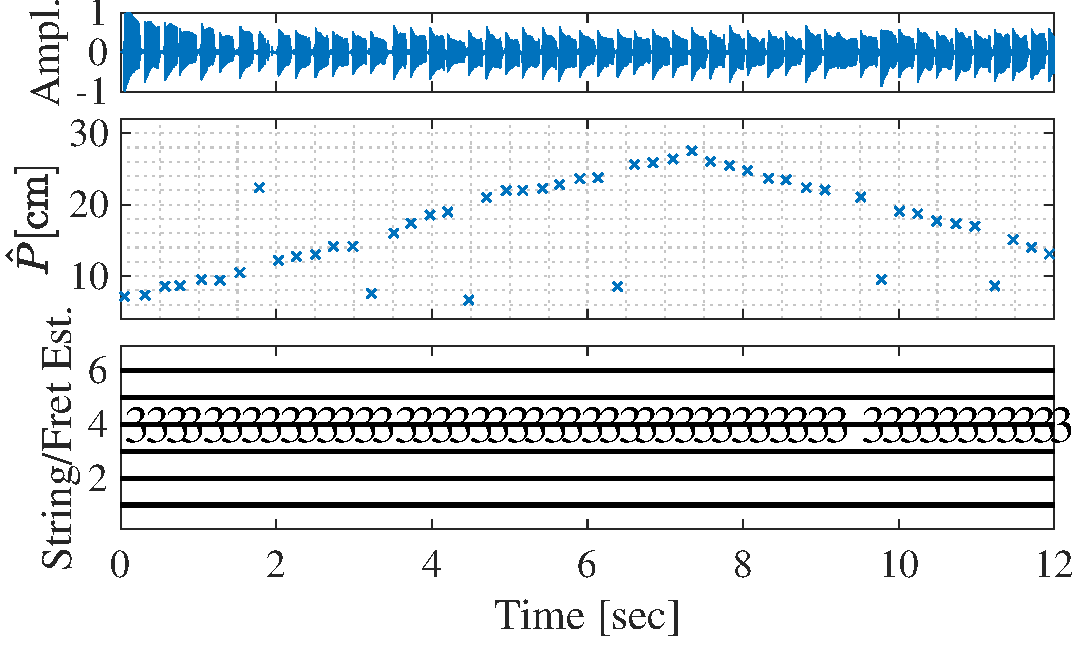
\includegraphics[width=.86\linewidth]{img/tablature_constant_note8}\vspace{-2mm}
   \caption{String, fret and plucking position estimates with moving plucking position and fixed string and fret for electric guitar.}
   \label{fig:pluck_position_fixed_tabs} 
\end{subfigure}
\vspace{4mm}
\begin{subfigure}
   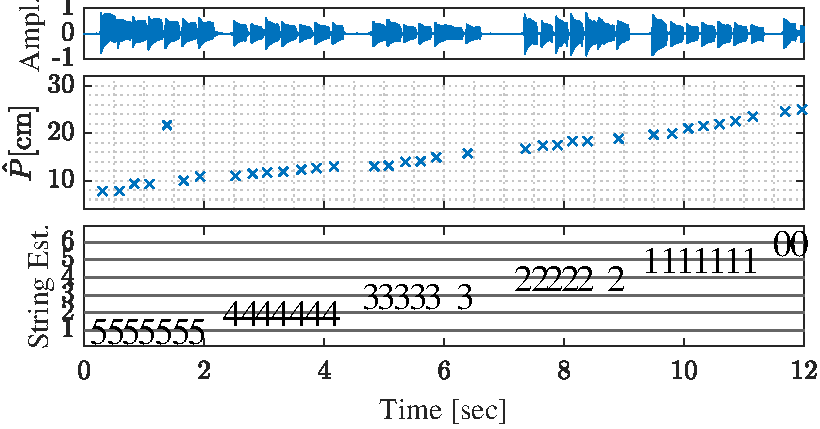
\includegraphics[width=.95\linewidth]{img/tablature_constant_note25_LSD}\vspace{-2mm}
   \caption{String, fret and plucking position estimates with moving plucking position and moving string and fret for electric guitar.}
   \label{fig:pluck_position_varied_tabs}
\end{subfigure}
\end{figure}
%
\section{Conclusion}
%
% -------------------------------------------------------------------------
% Either list references using the bibliography style file IEEEtran.bst
\bibliographystyle{IEEEtran}
\bibliography{myabbr,refs17,refs}
%
% or list them by yourself
% \begin{thebibliography}{9}
% 
% \bibitem{waspaa17web}
%   \url{http://www.waspaa.com}.
%
% \bibitem{IEEEPDFSpec}
%   {PDF} specification for {IEEE} {X}plore$^{\textregistered}$,
%   \url{http://www.ieee.org/portal/cms_docs/pubs/confstandards/pdfs/IEEE-PDF-SpecV401.pdf}.
%
% \bibitem{PDFOpenSourceTools}
%   Creating high resolution {PDF} files for book production with 
%   open source tools, 
%   \url{http://www.grassbook.org/neteler/highres_pdf.html}.
%
% \bibitem{eWilliams1999}
% E. Williams, \emph{Fourier Acoustics: Sound Radiation and Nearfield Acoustic
%   Holography}. London, UK: Academic Press, 1999.
% 
% \bibitem{ieeecopyright}
%   \url{http://www.ieee.org/web/publications/rights/copyrightmain.html}.
%
% \bibitem{cJones2003}
% C. Jones, A. Smith, and E. Roberts, ``A sample paper in conference
%   proceedings,'' in \emph{Proc. IEEE ICASSP}, vol. II, 2003, pp. 803--806.
% 
% \bibitem{aSmith2000}
% A. Smith, C. Jones, and E. Roberts, ``A sample paper in journals,'' 
%   \emph{IEEE Trans. Signal Process.}, vol. 62, pp. 291--294, Jan. 2000.
% 
% \end{thebibliography}


\end{sloppy}
\end{document}
